%\documentclass[handout]{beamer}
\documentclass{beamer}

\usetheme{Madrid}
\usecolortheme{whale}
\useinnertheme{circles} 
\useoutertheme{split}
\setbeamertemplate{blocks}[rounded][shadow=true]

\usepackage[OT2,T1]{fontenc}
\usepackage[utf8]{inputenc}
\usepackage{lmodern}
\usepackage{amsfonts,amsmath,amssymb,amsthm}
\usepackage{colortbl}
\usepackage[all]{xy}
\usepackage{tikz-cd}
\usepackage{hyperref}
\usepackage[backend=bibtex,style=authoryear, defernumbers=true]{biblatex}

\addbibresource{citations.bib}
%\beamertemplatenavigationsymbolsempty

\title{Algebras for a Functor}
\author[Gašper, Nejc]{Gašper Golob and Nejc Zajc}
%\institute{University of Ljubljana, Slovenia}
\date{Project presentation, 26.5.2022}



\begin{document}
%%%%%%%%%%%%%%%%%%%%%%%%%%%%%%%%%%%%%%%%
\begin{frame}
\maketitle

\end{frame}
%%%%%%%%%%%%%%%%%%%%%%%%%%%%%%%%%%%%%%%%
\begin{frame}
\frametitle{Motivation}

Modelling inductive types.


\end{frame}
%%%%%%%%%%%%%%%%%%%%%%%%%%%%%%%%%%%%%%%%
\begin{frame}[fragile]
\frametitle{F-Algebras}

category $C$, endofunctor $F \colon C \to C$
\\~\\
\pause


\[
\begin{tikzcd}[transform canvas={scale=1.5}]
	{FA} && A 
	\arrow["\alpha", from=1-1, to=1-3]
\end{tikzcd}
\]

\end{frame}
%%%%%%%%%%%%%%%%%%%%%%%%%%%%%%%%%%%%%%%%
\begin{frame}[fragile]
\frametitle{F-Algebras}

category $C$, endofunctor $F \colon C \to C$
\\~\\~\\~\\

\[
\begin{tikzcd}[transform canvas={scale=1.5}]
	{FA} && A \\
	\\
	{FB} && B
	\arrow["\alpha", from=1-1, to=1-3]
	\arrow["{Ff}"', from=1-1, to=3-1]
	\arrow["\beta", from=3-1, to=3-3]
	\arrow["f", from=1-3, to=3-3]
\end{tikzcd}
\]

\end{frame}
%%%%%%%%%%%%%%%%%%%%%%%%%%%%%%%%%%%%%%%%
\begin{frame}
\frametitle{Initial Objects}

Such an object $I$, that for every object $X$, \\ there exist a \textbf{unique} morphism $I \to X$.

\end{frame}
%%%%%%%%%%%%%%%%%%%%%%%%%%%%%%%%%%%%%%%%
\begin{frame}[fragile]
\frametitle{Lambek Lemma}
\begin{lemma}[Lambek]
If $I = (A, \alpha)$ is an initial algebra, then $A$ is isomorphic to $FA$ via $\alpha$.
\end{lemma}
\quad \\~\\~\\
\pause

\[
\begin{tikzcd}[transform canvas={scale=1.5}]
	FA && A \\
	\\
	{F(FA)} && FA
	\arrow["\alpha", from=1-1, to=1-3]
	\arrow["Fi"', from=1-1, to=3-1]
	\arrow["F\alpha", from=3-1, to=3-3]
	\arrow["i", from=1-3, to=3-3]
\end{tikzcd}
\]

\end{frame}
%%%%%%%%%%%%%%%%%%%%%%%%%%%%%%%%%%%%%%%%
\begin{frame}
\frametitle{Polynomial Functor}
\begin{itemize}
\item project only defines them on \textbf{Sets}
\item \( PX = \sum_{i \in I}X^{A_i} \), for \(A : I \to \textbf{Set}\)
\item natural numbers from \(PX = 1 + X\)
\end{itemize}


\end{frame}
%%%%%%%%%%%%%%%%%%%%%%%%%%%%%%%%%%%%%%%%
\begin{frame}[fragile]
\frametitle{Initial algebra for polynomial functors}
\begin{itemize}
\item \(\text{Tree}\) has a constructor \(\text{Node } \sum_{i\in I}\text{Tree}^{A_i}\)
\item initial object is the F-algebra of the Tree
  % https://q.uiver.app/?q=WzAsNCxbMCwwLCJcXHN1bV97aVxcaW4gSX1cXHRleHR7VHJlZX1ee0FfaX0iXSxbMiwwLCJcXHRleHR7VHJlZX0iXSxbMCwyLCJQQj1cXHN1bV97aSBcXGluIEl9Ql57QV9pfSJdLFsyLDIsIkIiXSxbMCwxLCJcXGFscGhhIl0sWzAsMiwiUGYiLDJdLFsyLDMsIlxcYmV0YSIsMl0sWzEsMywiZiJdXQ==
  \[\begin{tikzcd}
      {\sum_{i\in I}\text{Tree}^{A_i}} && {\text{Tree}} \\
      \\
      {\sum_{i \in I}B^{A_i}} && B
      \arrow["\alpha", from=1-1, to=1-3]
      \arrow["Pf"', from=1-1, to=3-1]
      \arrow["\beta"', from=3-1, to=3-3]
      \arrow["f", from=1-3, to=3-3]
    \end{tikzcd}\]
\end{itemize}

\end{frame}

%%%%%%%%%%%%%%%%%%%%%%%%%%%%%%%%%%%%%%%%
\begin{frame}
\frametitle{Future work}
\begin{itemize}
\item implement presentation of natural numbers with F-algebras
\item implement presentation of lists with F-algebras
\item generalize polynomial functors
\item generalize existance of initial algebras
\end{itemize}


\end{frame}
%%%%%%%%%%%%%%%%%%%%%%%%%%%%%%%%%%%%%%%%
\begin{frame}
\frametitle{Problems in Implementation}

\pause

\begin{figure}[h]
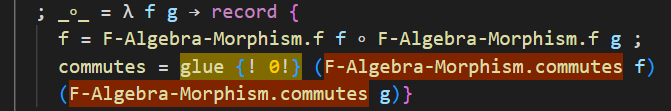
\includegraphics[width=12cm]{yellow.PNG}
\end{figure}


\end{frame}

%%%%%%%%%%%%%%%%%%%%%%%%%%%%%%%%%%%%%%%%
\begin{frame}
  \frametitle{Sources}
  \nocite{*}
  \printbibliography
\end{frame}



%%%%%%%%%%%%%%%%%%%%%%%%%%%%%%%%%%%%%%%%
\end{document}
